This section presents two case studies on real industrial-scale energy storages and a real data benchmark to demonstrate the effectiveness and applicability of our proposed approach. We investigate the properties and performance of the approach using signals from IoT devices in an energy system and streamed benchmark system data. The successful deployment demonstrates that this approach is suitable for existing industrial systems utilizing IoT data streams on top of well-established SCADA systems.

\subsection{Battery Energy Storage System TERRA}\label{AA:BESS}
In the first case study, we demonstrate our proposed method on real industrial-scale battery energy storage system (BESS) TERRA, depicted in Fig \ref{fig:terra}. TERRA has an installed capacity of 151 kWh distributed among 10 modules with 20 Li-ion NMC cells. The Inverter's nominal power is 100 kW.
The TERRA reports measurements of State of Charge (SoC), supply/draw energy set-points, and inner temperature, at 6 positions (channels) of each battery module. A substantial size of the system, which is 2.4x2.4x1.2m (HxWxD), requires a proper cooling mechanism. The cooling is handled by forced air from the HVAC system and inner fans, while the fire safety system is passive. Tight battery temperature control is needed to optimize performance and maximize the safety and battery's lifespan. Identifying anomalous events and removal of corrupted data might yield significant improvement in the process control level and increase the reliability and stability of the system.

\begin{figure}[htbp]
 \centering
 \resizebox{\linewidth}{!}{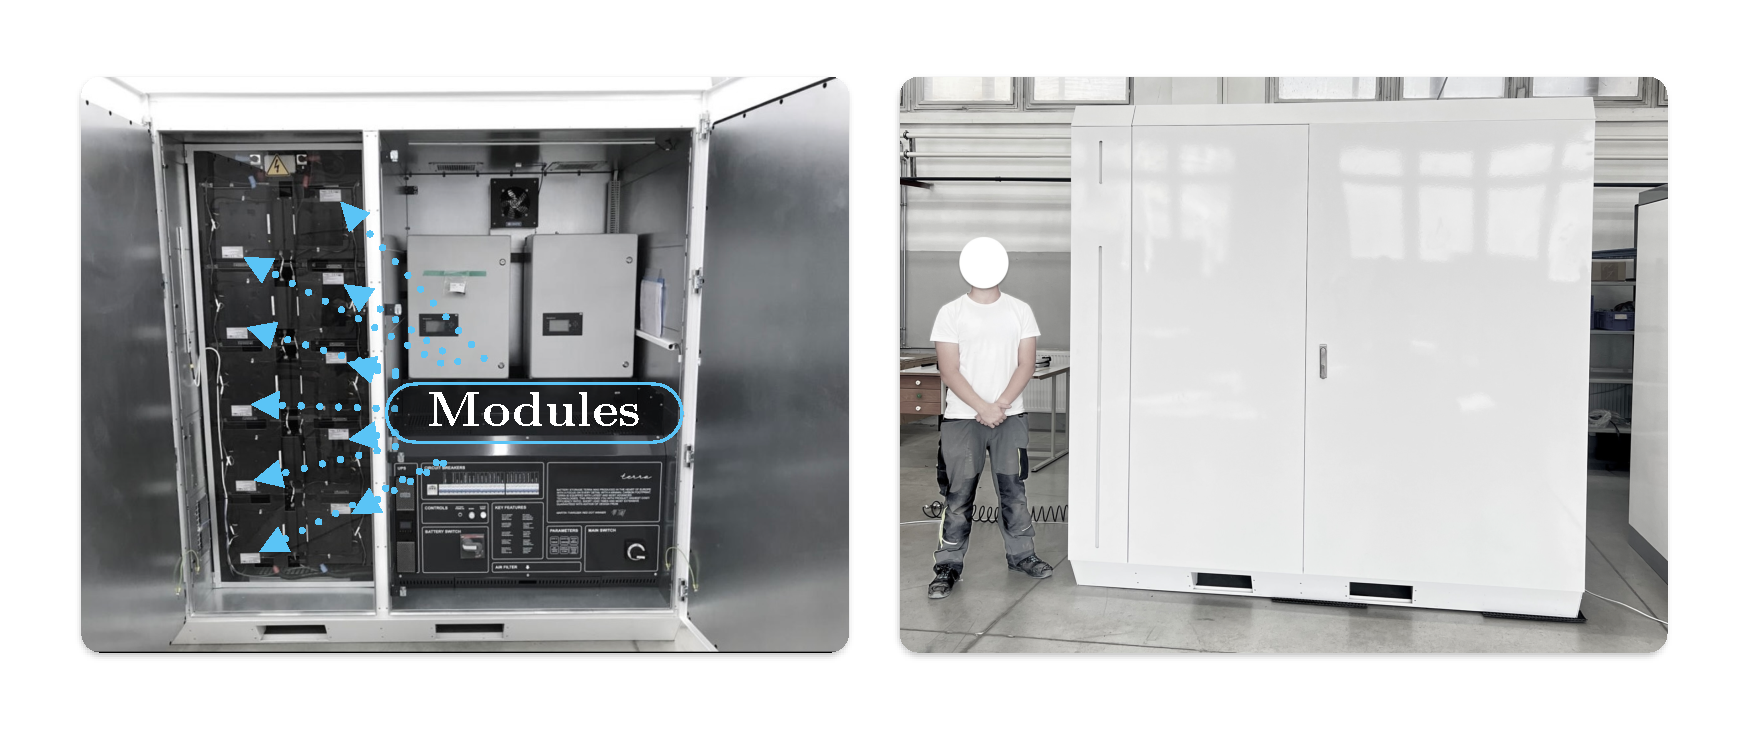
\includegraphics{figures/TERRA_PAPER.pdf}}
 \caption{Photograph of the actual studied TERRA energy storage unit with open doors (left), and closed doors (right).}
 \label{fig:terra}
\end{figure}

The AID is integrated into the existing software infrastructure of the system, allowing detection and diagnosis of the system using streamed IoT data. Here we replay a 9-day stream of historical measurements of the device, to demonstrate key features of AID.

For demonstration purposes, the expiration period $\ui{t}{e}$ is set to 4 days, as the system is expected to adapt to the new behavior, due to the transfer of the module to the outside. The grace period was reduced to 1 day, to observe the reaction to concept drift. The threshold $T$ is set to $3.5 \sigma$ to reduce the number of alarms. The frequency will be higher as the detector is protected and self-supervised. The adaptation period $\ui{t}{a}$ is changed to 3 hours as this is the time constant of the temperature to the unit change of supply/draw power demand.

Figure \ref{fig:terra_no_change} depicts the average cell temperature measurement of the TERRA for all 10 modules. The data are normalized to the range $[0, 1]$ to protect the sensitive business value. The light red area represents the region out of dynamic operating limits as provided by AID. On 7\textsuperscript{th} March 2022, the system was relocated from the inside of the building to the outside power socket. The system was expected to adapt to the new behavior within 4 days as specified by $\ui{t}{e}$. Nevertheless, due to the protection of the model from learning the anomalous data, the new behavior could not be captured as the system was not operating within the safe limits. The adaptation started three days later, as only some of the measurements within the safe region after transfer were learned. Therefore, the importance of self-supervised adaptation to changes in data is crucial. As we can see, the change points detection according to \eqref{eq:changepoint} alerted such change shortly after the TERRA was connected to a data broker, while the length of the adaptation period enabled discrimination from collective anomaly.

\begin{figure}
 \centering
 \resizebox{\linewidth}{!}{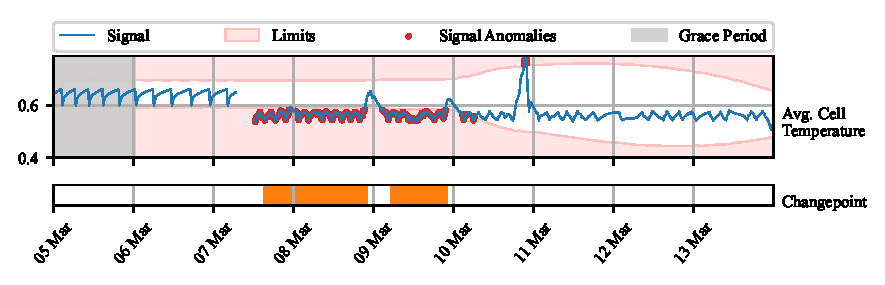
\includegraphics{figures/TERRA_thresh_single_4days_shift_no_change_adapt.pdf}}
 \caption{\replaced{Normalized average cell temperature of TERRA}{Time series of TERRA measurements} observed over 9 days (blue line).\deleted{ The y-axis renders the average temperature of all cells and modules after the normalization to the range of $[0, 1]$.} The \replaced{model \textbf{without} adaptation to change points holds dynamic operating limits (light red area) unchanged, and anomaly (red dots) alerted for approximately three days.}{light red area represents an area out of dynamic operating limits for individual signals. Observations out of the limits are marked by a red dot.} Orange bars represent the times, at which changepoints were detected. Grace period is grayed out.}
 \label{fig:terra_no_change}
\end{figure}

In Figure \ref{fig:terra_change} we depict the same measurement with a changepoint adaptation mechanism in place. The mechanism speeds up the adaptation to the new behavior, as the system is allowed to learn from anomalous data when they represent the changed behavior. The adaptation took approximately 6 times shorter.

\begin{figure}
 \centering
 \resizebox{\linewidth}{!}{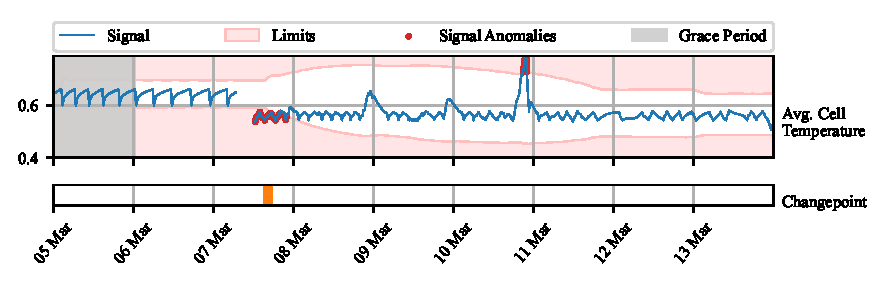
\includegraphics{figures/TERRA_thresh_single_4days_shift_change_adapt.pdf}}
 \caption{\replaced{Normalized average cell temperature of TERRA}{Time series of TERRA measurements} observed over 9 days (blue line).\deleted{ The y-axis renders the average temperature of all cells and modules after the normalization to the range of $[0, 1]$.} The \replaced{model \textbf{with} adaptation to change points starts to update dynamic operating limits (light red area) within 3 hours and alerts anomaly (red dots) for approximately 10 hours.}{light red area represents an area out of dynamic operating limits for individual signals. Observations out of the limits are marked by a red dot.} Orange bars represent the times, at which changepoints were detected. Grace period is grayed out.}
 \label{fig:terra_change}
\end{figure}

The default sampling rate of the incoming signal measurements is 1 minute. However, network communication of the IoT devices is prone to packet dropout, which results in unexpected non-uniformities in sampling from the perspective of the SCADA system. The transfer of TERRA was accompanied by the disconnection of IoT sensors from the data broker which might be considered an anomaly. The system can detect such anomalies as well, as depicted in Figure \ref{fig:terra_sampling}. Along with known disconnection, the system alerted two more non-uniformities of shorter extend, scaled in the figure for better visibility. The short loss of signal was caused by the packet drop, as it impacted only a few consecutive measurements. Various confidence levels could be used to further analyze and map potential causes to the duration of the outage.

\begin{figure}[htbp]
 \centering
 \resizebox{\linewidth}{!}{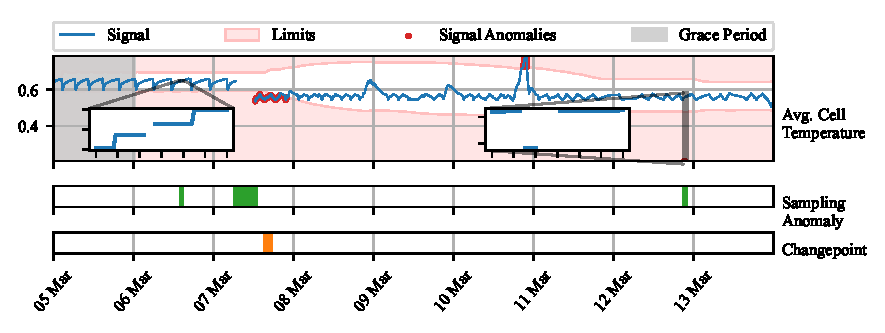
\includegraphics{figures/TERRA_thresh_single_4days_sampling.pdf}}
 \caption{\replaced{Normalized average cell temperature of TERRA}{Time series of TERRA measurements} observed over 9 days (blue line).\deleted{ The y-axis renders the average temperature of all cells and modules after the normalization to the range of $[0, 1]$.} The \replaced{model \textbf{with} adaptation to change points and sampling nonuniformity alerts}{light red area represents an area out of dynamic operating limits for individual signals. Observations out of the limits are marked by a red dot.}\added{ Green bars represent the times, at which sampling anomalies are detected, while zoomed areas focus on short events of abnormal sampling.} Orange bars represent the times, at which changepoints were detected. Grace period is grayed out.}
 \label{fig:terra_sampling}
\end{figure}

Lastly, we want to acknowledge the outlier, left uncaptured due to increased variance of the distribution in a period of adaptation. Observing multiple variables, where some might be influenced less by the change in behavior, might be beneficial in such cases. The industrial partner provided a physics-based model of the battery module temperature, defined as follows:
\begin{align}
 \uis{T}{bat}{i+1} &= \uis{T}{bat}{i} + \ui{T}{s} (\ui{q}{fan} \ui{V}{b,max} \rho \ui{c}{p} (\ui{T}{out} - \uis{T}{bat}{i}) + \ui{V}{c,max}\ui{q}{circ.fan} \rho \ui{c}{p} \uis{T}{bat}{i} \nonumber \\
 &+ \ui{q}{circ.fan} (\ui{P}{cool} \ui{q}{cool} \ui{P}{heat} \ui{q}{heat}) + \ui{c}{scale} \ui{Q}{bat} + \ui{q}{inner fans} \\
 &- (\ui{V}{b,max} \ui{q}{fan} \ui{V}{c,max} \ui{q}{circ.fan}) \rho \ui{c}{p} \uis{T}{bat}{i}) / (\ui{m}{bat} \ui{c}{p,b}) \text{}\nonumber
\end{align}

When combined with an averaged measurement of battery module temperature, we could compute the difference between real and predicted temperature. Such deviation can be useful in detecting unexpected patterns in temperature due to the impact of external disturbance and aging. Nevertheless, it may be inaccurate as the physics-based model is simplified and does not account for spatial aspects, like temperature gradients as well as different dynamic effects of charging and discharging on temperature. For instance, in Fig. \ref{fig:terra} during the first two days we see, that the cooling dynamic is not captured well, resulting in a subtle positive difference between average cell temperature and the temperature predicted by the model. In combination with the raw measured average of the temperature, the AID captures the outlier on 9\textsuperscript{th} March which could not be captured in a univariate setting. The physics-based model exposes temporal aspects of the behavior as it considers the dynamics of its inputs. The rapid increase in temperature w.r.t the modeled dynamics due to environmental conditions will draw a sharp positive peak in the difference between the real and predicted temperature, which will slowly vanish. Based on the significance of the deviation, the peak will be notified as a single-point anomaly or collective anomaly.

\begin{figure}[htbp]
\centerline{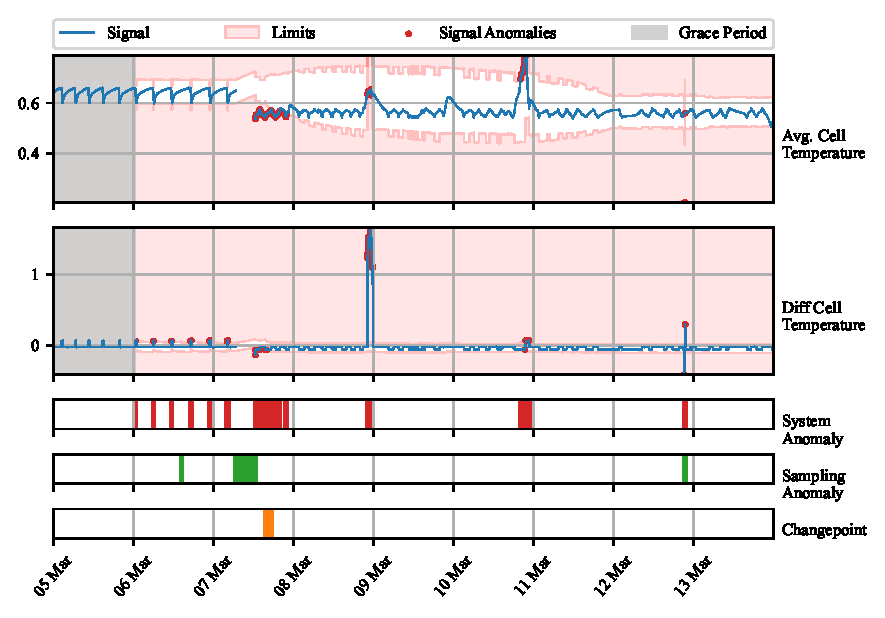
\includegraphics{figures/TERRA_thresh_4days.pdf}}
\caption{Time series of TERRA measurements observed over 9 days (blue line). The y-axis renders the average temperature of all cells and modules after the normalization to the range of $[0, 1]$. The light red area represents an area out of dynamic operating limits for individual signals. Observations out of the limits are marked by a red dot. Orange bars represent the times, at which changepoints were detected. Green bars represent periods where sampling anomaly was alerted. Red bars denote the period where any of the signals contained anomaly. Grace period is grayed out.}
\label{fig:terra_multi}
\end{figure}

This case study demonstrated AID's effectiveness  within the context of the energy storage system, specifically the TERRA system. The AID system exhibited adaptability to changes in the operational environment, contributing to its versatility and robustness. Additionally, it facilitated the establishment of dynamic operating limits for SCADA systems, considering context of the device such as environmental conditions or aging. Furthermore, the AID system showcased its capability to operate with a physics-based model, enhancing the precision of anomaly detection processes. This highlights the potential of AID as a valuable tool within complex industrial systems. The validity of our proposed approach was verified by our industrial partner, who confirmed that the detected anomalies were indeed caused by the aforementioned events.

\subsection{Kokam Battery Module}\label{AA:Kokam}
A second case study presents temperature profile monitoring of individual modules of battery pack TERRA deployed at the premises of the end user. During the operation, a hardware fault of module's 9 cooling fan occurred on 23\textsuperscript{rd} August 2023 at 17:12:30. Our industrial partner was interested in finding out, whether such an event could be captured by an anomaly detection system. Each of the 10 modules, embodies 20 cells measured by 6 spatially distributed sensors as shown in Figure \ref{fig:kokam_module}. The measurements are sent in 30-second intervals and processed in a streamed manner by SCADA. With the availability of the temperature profiles for all the modules, we computed the deviation of the observed value from the average of all the modules' temperature measurements. The ground truth information about the fan fault was provided to the best of the operator's knowledge. However, this information serves for evaluation only, as the system operates in a self-supervised manner.

\begin{figure}[htbp]
\centering
 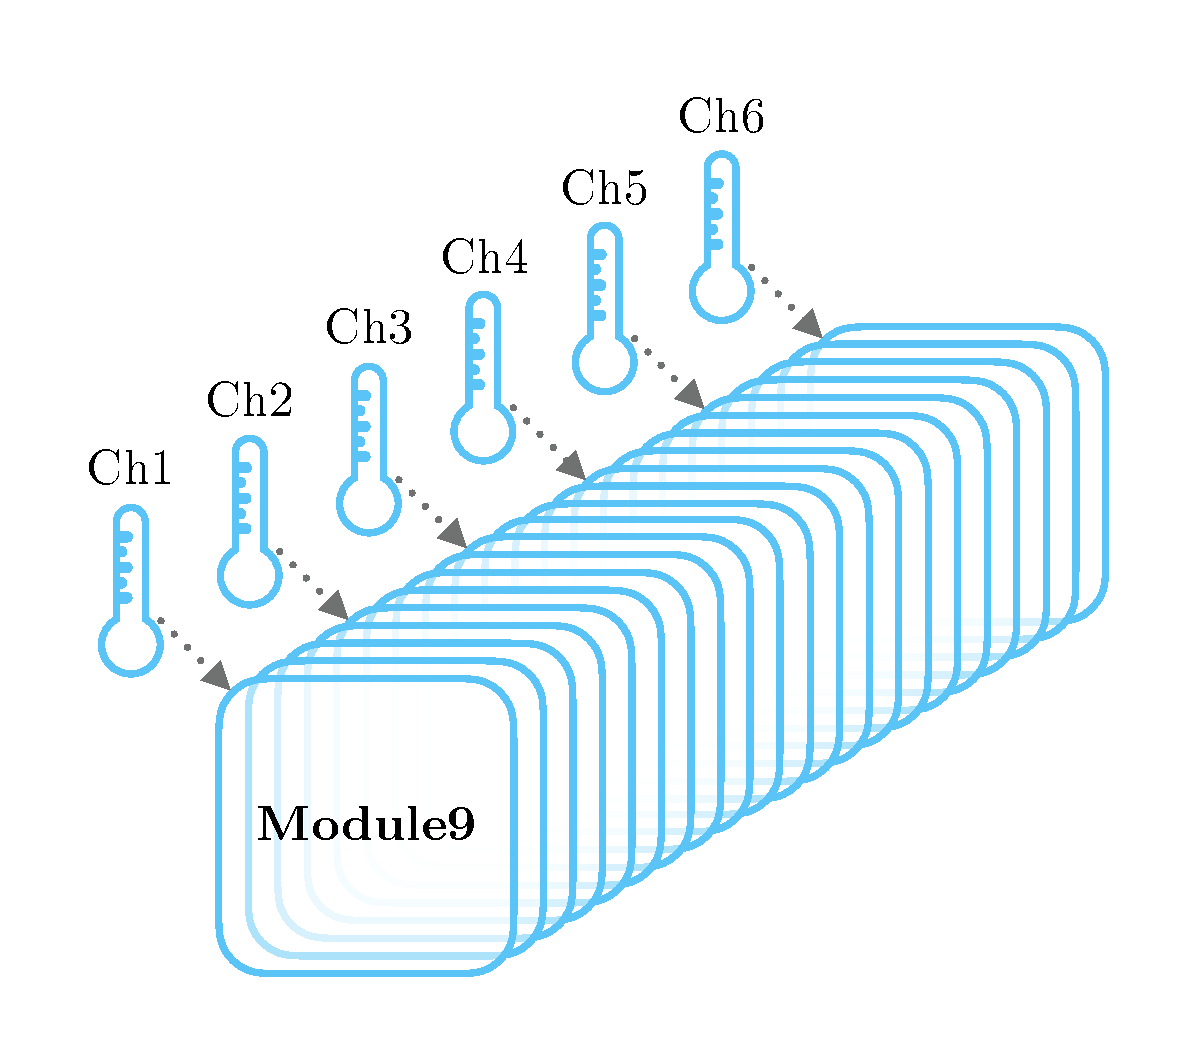
\includegraphics[width=0.6\textwidth]{figures/Kokam_module9_measure points.pdf}
 \caption{Module 9 with 20 cells and 6 sensors measuring the temperature at each 4\textsuperscript{th} cell.}
 \label{fig:kokam_module}
\end{figure}

Our anomaly detection system was, in this case, initialized for the operation in production. The expiration period of 7 days, allowed the system to adapt to weekly seasonality due to the usage of the battery following work week. The grace period was kept at the default value, equal to $\ui{t}{e}$. The threshold value was shifted to a 4 sigma value of 99.977\% which makes the the frequency of anomalous events approximately once a week given 30-second sampling. The adaptation period was held constant as the deployed system is not expected to change its behavior dramatically on a daily basis.

In Figure \ref{fig:kokam_first} we observe 4 days of operation around the period of fan fault occurrence. The deviations between the observed temperature measured by channels of module 9 and the average temperature of all modules are displayed. The dynamic operating limits tightly envelop temperatures measured by the sensors in the middle of the module (refer to Figure \ref{fig:kokam_module}), while measurements at both sides deviate more due to the proximity to the walls and sources of disturbance. We observed multiple alarms raised by various channels individually before the fan fault. These anomalies, while not addressed here further, could be subjects of interest for further investigation by system operators. Meanwhile, the fan fault at the center of our focus is alarmed based on three measurements, namely channels 1, 2, and 3. From the zoomed views, we can observe a sharp increase in the temperature deviation. The alarm is on until 24\textsuperscript{th} August at noon, when significant fluctuations vanish followed by temporary settling of the temperature. On 25\textsuperscript{th} August at 11:21, increased temperature fluctuations are followed by an increase of temperature similar to the initial one.
AID alerts this fault again based on measurements by channels 1, 2, and 3.

\begin{figure}[htbp]
 \centerline{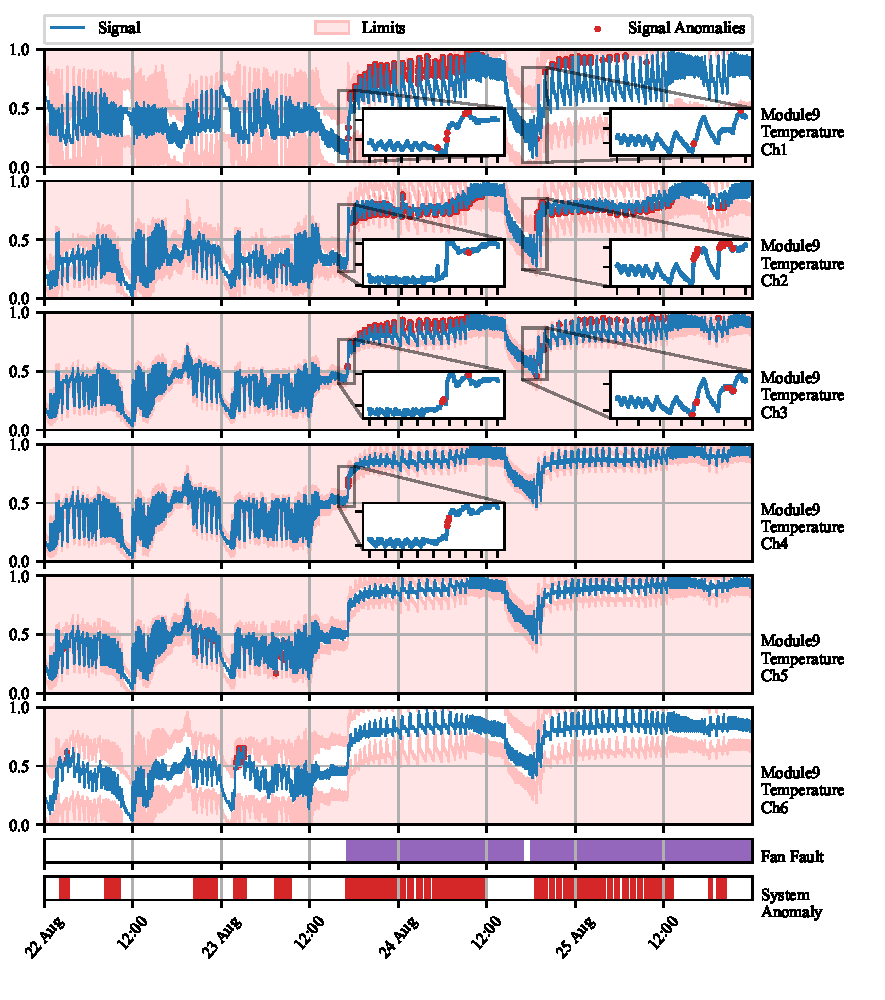
\includegraphics{figures/Kokam_thresh_first_zoom.pdf}}
 \caption{Time series of battery module 9 measurements (blue line). The y-axis renders the normalized deviations of temperature from the average of all modules. Signal anomalies are marked as red dots. The light red area represents an area out of dynamic operating limits. True fan faults are marked by purple bars. Green bars represent the times of changepoint detection. Red bars denote the period where any signal anomaly.}
 \label{fig:kokam_first}
\end{figure}

Time series of TERRA measurements observed over 9 days (blue line). The y-axis renders the average temperature of all cells and modules after the normalization to the range of $[0, 1]$. The light red area represents an area out of dynamic operating limits for individual signals. Observations out of the limits are marked by a red dot. Orange bars represent the times, at which changepoints were detected. Green bars represent periods where sampling anomaly was alerted. Red bars denote the period where any of the signals contained anomaly. Grace period is grayed out.

Interestingly, during the presence of a fault in the fan, two more periods where the fan started operating again followed as depicted in Figure \ref{fig:kokam_second}. Periods of operation were interrupted again on 27\textsuperscript{th} and 28\textsuperscript{th} August respectively in the early morning hours. In both of the cases, AID detected the presence of the fault at the moment of occurrence. In the first case, channel 3 reported an anomaly slightly before the increase in temperature, due to abnormal fluctuation happening prior to faults.

\begin{figure}[htbp]
 \centerline{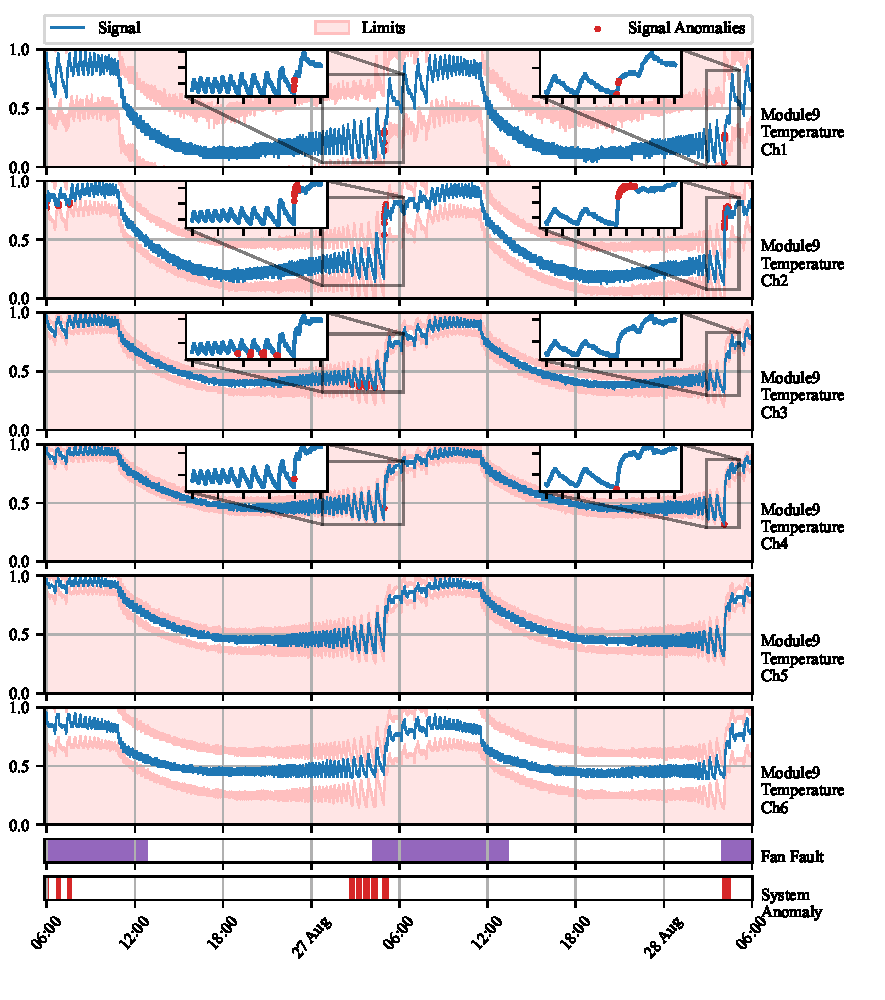
\includegraphics{figures/Kokam_thresh_second_zoom.pdf}}
 \caption{Time series of battery module 9 measurements (blue line). The y-axis renders the normalized deviations of temperature from an average of all modules. Signal anomalies are marked as red dots. The light red area represents an area out of dynamic operating limits. True fan faults are marked by purple bars. Green bars represent the times of changepoint detection. Red bars denote the period where any of the signals contained anomaly.}
 \label{fig:kokam_second}
\end{figure}

This case study demonstrates the effectiveness of the AID framework in identifying hardware faults within the context of energy storage systems. It showcases the system's ability to harness spatially distributed sensors that measure the same process variable. The AID system successfully pinpointed a fault in a cooling fan during real-world production operations, underlining its practical utility and its relevance in enhancing the safety of energy storage systems. Furthermore, the incorporation of adaptation mechanisms ensures that the system can be deployed over extended periods without necessitating resource-intensive retraining. Additionally, the concept of dynamic operating limits introduced in this study holds promise for integration with Supervisory Control and Data Acquisition (SCADA) monitoring systems, enabling proactive responses in situations where human life, equipment, or the environment may be at risk.

\subsection{Real Data Benchmark}\label{AA:Benchmark}
% The case studies were realized using Python 3.10.1 on a machine employing an 8-core Apple M1 CPU and 8 GB RAM.
The benchmarking comparison in this subsection evaluates the AID framework against adaptive unsupervised detection methods, specifically One-Class Support Vector Machine (OC-SVM) and Half-Space Trees (HS-Trees). These methods are widely recognized for their iterative learning capabilities on multivariate time-series data, making them suitable for anomaly detection in dynamic systems, as previously discussed in the Introduction \ref{par:validation}.

The comparison is based on the Skoltech Anomaly Benchmark (SKAB) dataset, a real-world dataset with annotated labels distinguishing between anomalous and normal observations \citep{skab2020}. SKAB is used for this purpose, as no established benchmarking multivariate data were found regarding energy storage systems similar to the ones studied in Subsection \ref{AA:BESS} and Subsection \ref{AA:Kokam}. The SKAB dataset involves experiments related to rotor imbalance, where various control actions and changes in water volume are introduced to the system. It encompasses eight features and exhibits both gradual and sudden drifts.

To ensure fairness in the benchmark, data preprocessing adheres to best practices for each method. OC-SVM employs standard scaling, while HS-Trees use normalization. Our proposed AID method requires no scaling. Preprocessing is performed online, simulating a real production environment, with running mean and variance for standard scaling and running peak-to-peak distance for normalization, as supported by the online machine learning library "river" \citep{Montiel2021}.

The optimal hyperparameters for both reference methods are found using Bayesian Optimization. Due to no further knowledge about the data generating process, and equity in benchmark, the hyperparameters of our proposed method were optimized using Bayesian Optimization as well. 20 steps of random exploration with 100 iterations of Bayesian Optimization were used, increasing default values set in the Bayesian Optimization library, to allow thorough exploration and increase the possibility of finding global optima in each case \citep{Nogueira2014}. The hyperparameters are optimized with the F1 score as a cost function first, to maximize both precision and recall on anomalous samples. % Second, the hyperparameters are optimized with macro F1 score, as it considers performance on both anomalous samples as well as normal samples equally. Therefore, the performance in the second case is not indifferent towards type I. errors, and false alarms due to the wrong detection of normal data as anomalies.

As adaptation is required and anticipated within benchmark datasets, the performance is evaluated iteratively, similarly to the operation after deployment. The metric is updated with each new sample and its final value is used to drive Bayesian Optimization. The performance is evaluated using the best-performing model, found by Bayesian Optimization. The performance of the proposed method is evaluated on the same data as the models are optimized for.

Hyperparameter search ranges are specified, with values centered around default library values for OC-SVM and HS-Trees. The ranges are intentionally set wide to facilitate comprehensive exploration. The quantile filter threshold used in OC-SVM and HS-Trees aligns with the threshold used in AID. These hyperparameter ranges are presented in Table \ref{tab:hyperparam_ranges}.

\begin{table}[ht]
\centering
\caption{Hyperparameter Ranges for Detection Algorithms}
\label{tab:hyperparam_ranges}
\begin{tabular}{|l|l|c|c|}
\hline
\textbf{Algorithm} & \textbf{Hyperparameters} & \textbf{Default} & \textbf{Ranges} \\
\hline
AID &
\begin{tabular}[c]{@{}l@{}}Threshold\\$\ui{t}{e}$\\$\ui{t}{a}$\\$\ui{t}{g}$\end{tabular} &
\begin{tabular}[c]{@{}c@{}}0.99735\\-\\$\ui{t}{e}$\\$\ui{t}{e}$\end{tabular} &
\begin{tabular}[c]{@{}c@{}}(0.85, 0.99994)\\(150, 10000)\\(50, 2000)\\(50, 1000)\end{tabular} \\
\hline
OC-SVM &
\begin{tabular}[c]{@{}l@{}}Threshold\\Learning Rate\end{tabular} &
\begin{tabular}[c]{@{}c@{}}-\\0.01\end{tabular} &
\begin{tabular}[c]{@{}c@{}}(0.85, 0.99994)\\(0.005, 0.02)\end{tabular} \\
\hline
HS-Trees &
\begin{tabular}[c]{@{}l@{}}Threshold\\N Trees\\Max Height\\Window Size\end{tabular} &
\begin{tabular}[c]{@{}c@{}}-\\10\\8\\250\end{tabular} &
\begin{tabular}[c]{@{}c@{}}(0.85, 0.99994)\\(0, 20)\\(2, 14)\\(100, 400)\end{tabular} \\
\hline
\end{tabular}
\end{table}


The results for models optimized for the F1 score are summarized in Table \ref{tab:perf_comp_f1}, which includes precision, recall, F1 score, and average latency. Macro values are enclosed in brackets, representing the mean of the metric for both anomalies and normal data. A perfect detection achieves 100\% in each metric \added{but false positive rate (FAR), where perfect detector achieves 0\%}. According to the Scoreboard for various algorithms on SKAB's Kaggle page, all iterative approaches perform comparably to the batch-trained isolation forest and autoencoder, validating the optimization process. Notably, the proposed AID method outperforms both reference methods in terms of \replaced{precision, recall, F1 score, area under curve, and false positive rate}{F1 score, recall, and precision}, despite having a 30-fold higher latency per sample. This highlights the scalability as a candidate for further development. Nevertheless, in this case, sampling of the benchmark data still offers enough time to deliver predictions with sufficient frequency.

\begin{table}[htbp]
    \caption{Evaluation of models optimized for F1 score on SKAB dataset \citep{skab2020}. The best-performing model is highlighted in bold. Values in brackets represent macro values of the metric.}
    \begin{center}
        \label{tab:perf_comp_f1}
        \begin{tabular}{|l|c|c|c|c|}
            \hline
            \textbf{Algorithm}              & AID                       & HS-Trees            & OC-SVM              \\
            \hline
            Precision [$\%$]                & $\boldsymbol{41}$ (59)    & 36 (51)             & 39 (54)             \\
            \hline
            Recall [$\%$]                   & $\boldsymbol{80}$ (59)    & 74 (51)             & 63 (54)             \\
            \hline
            F1 [$\%$]                       & $\boldsymbol{54}$ (53)    & 48 (44)             & 48 (52)             \\
            \hline
            \added{AUC [$\%$]}              & \added{$\boldsymbol{59}$} & \added{51}          & \added{54}          \\
            \hline
            \added{Mean Rolling AUC [$\%$]} & \added{$\boldsymbol{57}$} & \added{50}          & \added{53}          \\
            \hline
            \added{FPR [$\%$]}              & \added{$\boldsymbol{47}$} & \added{56}          & \added{48}          \\
            \hline
            Avg. Latency [ms]               & 1.45                      & $\boldsymbol{0.05}$ & $\boldsymbol{0.05}$ \\
            \hline
        \end{tabular}
    \end{center}
\end{table}

Optimal hyperparameters found during Bayesian Optimization are detailed in Table \ref{tab:hyperparam_f1}. None of the parameters are at the edge of the provided ranges, serving as necessary proof of ranges being broad enough. Nevertheless, sufficient proof is not possible as multiple parameter ranges are not bounded by designed limits.

\begin{table}[ht]
    \centering
    \caption{Optimal hyperparameters of methods optimized for F1 score}
    \label{tab:hyperparam_f1}
    \begin{tabular}{|l|l|c|}
        \hline
        \textbf{Algorithm}                                                                       & \textbf{Hyperparameters} & \textbf{Found} \\
        \hline
        AID                                                                                      &
        \begin{tabular}[c]{@{}l@{}}Threshold\\$\ui{t}{e}$\\$\ui{t}{a}$\\$\ui{t}{g}$\end{tabular} &
        \begin{tabular}[c]{@{}c@{}}0.96442\\1136\\396\\546\end{tabular}                                                                      \\
        \hline
        OC-SVM                                                                                   &
        \begin{tabular}[c]{@{}l@{}}Threshold\\Learning Rate\end{tabular}                         &
        \begin{tabular}[c]{@{}c@{}}0.86411\\0.01956\end{tabular}                                                                             \\
        \hline
        HS-Trees                                                                                 &
        \begin{tabular}[c]{@{}l@{}}Threshold\\N Trees\\Max Height\\Window Size\end{tabular}      &
        \begin{tabular}[c]{@{}c@{}}0.99715\\1\\7\\283\end{tabular}                                                                           \\
        \hline
    \end{tabular}
\end{table}

\subsection{Scalability Analysis}\label{AA:Scalability}

The scalability of the proposed method is evaluated on the temperature data of 10 battery modules with 6 points of temperature measurements in the TERRA system. The data are sampled at 30 second intervals and streamed to the AID system. The AID system is initialized with the same parameters as in Subsection \ref{AA:Kokam}. The data are processed in a streamed manner, simulating the real production environment. The latency of the system is measured as the time between the arrival of the sample and the delivery of the prediction. The latency is measured on a machine with an 8-core Apple M1 CPU and 8 GB RAM. The latency is measured for 20160 samples from 2023-08-21 to 2023-08-27. The latency analysis is performed for detection task alone and for the combined task of detection and dynamic process limits establishmend. The results are depicted in Table \ref{tab:latency}.

\begin{table}[htbp]
    \caption{Latency analysis of the proposed method.}
    \begin{center}
        \label{tab:latency}
        \begin{tabular}{|l|c|c|}
            \hline
            \textbf{Features} & \begin{tabular}[c]{@{}c@{}}\textbf{Detection}\\$\mu \pm \sigma$ ($\min$, $\max$) [ms]\end{tabular} & \begin{tabular}[c]{@{}c@{}}\textbf{Detection + Limits}\\$\mu \pm \sigma$ ($\min$, $\max$) [ms]\end{tabular} \\
            \hline
            1 & $0.337 \pm 0.500~(0.100, 0.600)$ & $0.337 \pm 0.500~(0.100, 0.600)$ \\
            10 & & \\
            20 & & \\
            30 & & \\
            40 & & \\
            50 & & \\
            60 & & \\
            \hline
        \end{tabular}
    \end{center}
\end{table}

The time complexity of the detection task to number of features is cubic
